\chapter{Практическая часть}
\section{Задание \No{}3}
\begin{table}[H]
    \centering
    \caption{Результаты вычисления выражений задания \No{}1}
	\begin{tabular}{|c|c|}
 	\hline
    Выражение & Результат \\
 	\hline
 	(caadr '((blue cube) (red pyramid))) & red \\
 	\hline
 	(cdar '((abc) (def) (ghi))) & nil \\
 	\hline
    (cadr '((abc) (def) (ghi))) & (def) \\
 	\hline
    (caddr '((abc) (def) (ghi))) & (ghi) \\
 	\hline
	\end{tabular}
\end{table}
\section{Задание \No{}4}
\begin{table}[H]
    \centering
    \caption{Результаты вычисления выражений задания \No{}2}
	\begin{tabular}{|c|c|}
 	\hline
    Выражение & Результат \\
 	\hline
    (list 'Fred 'and 'Wilma) & (FRED AND WILMA) \\
 	\hline
    (list 'Fred '(and Wilma)) & (FRED (AND WILMA))\\
 	\hline
    (cons nil nil) & (NIL) \\
 	\hline
    (cons t nil) & (T) \\
 	\hline
    (cons nil t) & (NIL .T)\\
 	\hline
    (list nil) & (NIL) \\
 	\hline
    (cons '(t) nil) & ((T)) \\
 	\hline
    (list '(one two) '(free temp)) & ((ONE TWO) (FREE TEMP)) \\
 	\hline
    (cons 'Fred '(and Wilma)) & (FRED AND WILMA) \\
 	\hline
    (cons 'Fred '(Wilma)) & (FRED WILMA) \\
 	\hline
    (list nil nil) & (NIL NIL) \\
 	\hline
    (list t nil) & (T NIL) \\
 	\hline
    (list nil t) & (NIL T) \\
 	\hline
    (cons t (list nil)) & (T NIL) \\
 	\hline
    (list (t) nil) & ((T) NIL) \\
 	\hline
    (cons '(one two) '(free temp)) & ((ONE TWO) FREE TEMP) \\
 	\hline
	\end{tabular}
\end{table}


\section{Задание \No{}5}
В листинге 2.1 приведён текст первой функции.

\lstset{language=lisp}
\begin{lstlisting}[caption={Примеры первой функции}]
(defun f1 (ar1 ar2 ar3 ar4)
  (list (list ar1 ar2) (list ar3 ar4))
)

(defun f1 (a1 a2 a3 a4)
    (cons (cons a1 (cons a2 Nil)) (cons (cons a3 (cons a4 Nil)) Nil))
)

; ((ar1 ar2) (ar3 ar4))
\end{lstlisting}

\par
В листинге 2.2 приведён текст второй функции.


\begin{lstlisting}[caption={Примеры второй функци}]
(defun f2 (ar1 ar2)
  (list (list ar1) (list ar2))
)

(defun f2 (a1 a2)
    (cons (cons a1 Nil) (cons (cons a2 Nil) Nil))
)

; ((ar1) (ar2))
\end{lstlisting}

\begin{lstlisting}[caption={Примеры второй функци}]
(defun f3 (a)
	(list (list (list a)))
)

(defun f3 (a)
    (cons (cons (cons a Nil) Nil) Nil)
)

; (((ar1)))
\end{lstlisting}

На рисунках 2.1-2.3 изображены списочные ячейки результатов рассмотренных выше функций.
\begin{figure}[H]
    \centering
    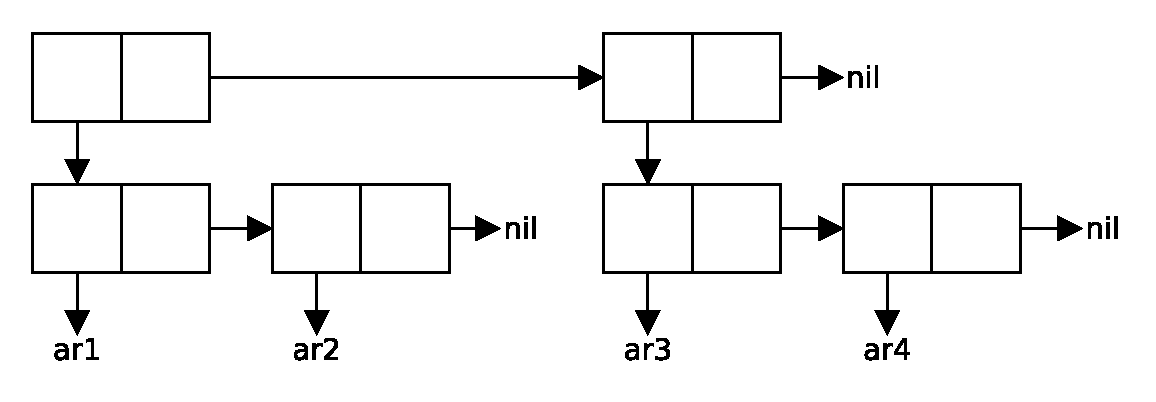
\includegraphics[scale=0.60]{data/pdf/02-01.pdf}
    \caption{Список ((ar1 ar2) (ar3 ar4))}
\end{figure}

\begin{figure}[H]
    \centering
    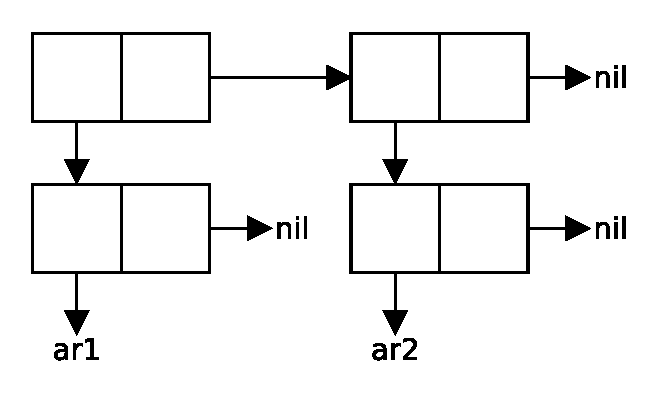
\includegraphics[scale=0.60]{data/pdf/02-02.pdf}
    \caption{Список ((ar1) (ar2))}
\end{figure}

\begin{figure}[H]
    \centering
    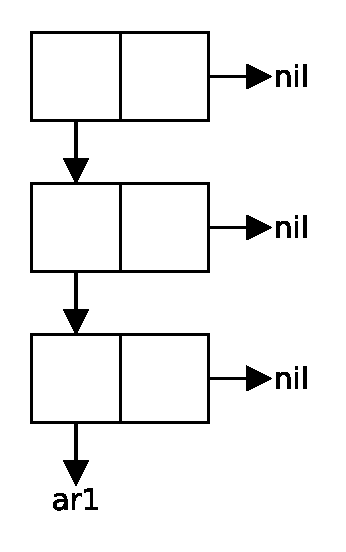
\includegraphics[scale=0.60]{data/pdf/02-03.pdf}
    \caption{Список (((ar1)))}
\end{figure}
